\documentclass{beamer}
%\documentclass[handout]{beamer}

\usepackage[latin1]{inputenc}
\usepackage{pifont}

\usecolortheme{albatross}

\mode<presentation>
{ 
    \usetheme{boxes} 
}


\title{Introduction to the semantic web \\ 
or \\
tripping with triples\ldots}
\author{
Pascal Mainini\\
\texttt{pascal <at> impressionet <dot> ch}\\
}
\date{2008-07-05}

\AtBeginSection[]
{
    \begin{frame}<beamer> 
        \frametitle{Outline}
        \tableofcontents[currentsection]
    \end{frame}
}

\begin{document}

    \begin{frame}
        \titlepage
    \end{frame}

    \section{Introduction}

        \begin{frame}
            \frametitle{About me}

            Before we start - some words about myself...
            \vskip 0.7cm
            \pause

            \begin{itemize}
                \item I'm Pascal Mainini
                \pause
                \item I'm also known as gurke 
                \pause
                \item Open minded, critical hacker
                \pause
                \item Started with computers almost 20 years ago, working professionally since nearly 10 years
                \pause
                \item Currently network and security specialist
                \pause
                \item \textit{I don't like beeing photographed or recorded otherwise, thanks!}
            \end{itemize}
        \end{frame}

        \begin{frame}
            \frametitle{About this speech}

            This speech will
            \vskip 0.7cm
            \pause

            \begin{itemize}
                \item Give an idea of what the semantic web is about
                \pause
                \item Give an overview of underlying technologies
                \pause
                \item Serve as a starting point for further explorations of the semantic web
            \end{itemize}
        \end{frame}

        \begin{frame}
            \frametitle{About this speech}

            This speech will \textbf{NOT}
            \vskip 0.7cm
            \pause

            \begin{itemize}
                \item Provide an exact mathematical background (I'm too lame for that...)
                \pause
                \item Give an in-depth tutorial of the technologies used (URIs, XML, RDF...)
                \pause
                \item Allow you to start working with semweb-technologies without investing any further work
            \end{itemize}
        \end{frame}

        \begin{frame}
            \frametitle{About this speech}

            This speech and additional material is licensed under a ``Attribution-Noncommercial-Share Alike 3.0 Unported'' license:
            \vskip 0.4cm

            \texttt{http://creativecommons.org/licenses/by-nc-sa/3.0/}
            \vskip 0.7cm

            The slides and additional material can (soon) be found at:
            \vskip 0.4cm

            \texttt{http://impressionet.ch/semwebspeech2}
            \vskip 2cm

            \begin{center}
                
\includegraphics[scale=0.5]{somerights}
            \end{center}
        \end{frame}

        \begin{frame}
            \frametitle{Prerequisites}

            To understand the examples in this speech, you will need a basic understanding of
            \vskip 0.7cm
            \pause

            \begin{itemize}
                \item URIs 
                \pause
                \item XML and XML namespaces
                \pause
                \item a bit of XML DTDs and schema
                \pause
            \end{itemize}
            \vskip 0.7cm
            \textbf{If you have questions, just ask them right away during the speak!}

        \end{frame}

    \section{The idea behind the semantic web}

        \begin{frame}
            \frametitle{Problems of the current web}

            The web as we know of it today has some problems\ldots
            \vskip 0.7cm
            \pause

            \begin{itemize}
                \item A gigantic bunch of information, a large diversity of formats
                \pause
                \item This information is stored in a form understandable for humans (which is great!)
                \pause
                \item It's not that easy for a machine to understand\ldots 
                \pause
                \item Thus, information is hard to find and reuse
            \end{itemize}
        \end{frame}

        \begin{frame}
            \frametitle{Solution approaches}

            To solve these problems, two possible ways exist:
            \vskip 0.7cm
            \pause

            \begin{itemize}
                \item Either, improve the usage of what's already there
                \pause
                \begin{itemize}
                    \item By improving techniques, especially artificial intelligence
                    \pause
                    \item This is hard to accomplish and the results so far aren't satisfying
                    \pause
                \end{itemize}
                \item Or by providing the information in a way better understandable by machines
                \pause
                \begin{itemize}
                    \item This requires standardised formats
                    \pause
                    \item These must be formally correct, simple and easily extensible
                \end{itemize}
            \end{itemize}
        \end{frame}

        \begin{frame}
            \frametitle{The semantic web}

            This is where the idea of the semantic web comes in.
            \vskip 0.3cm
            A full set of standards to accomplish this has been created by the W3C.
            \vskip 0.3cm
            Technologies used base (not exclusively) on \textbf{XML} and \textbf{URI}s as discussed before.
            \vskip 0.3cm
            On top of these follow \textbf{RDF}, \textbf{rdfschema} and \textbf{OWL}.
            \vskip 0.3cm
            This is called the \textit{semantic web layer cake}, let's have look at it\ldots
        \end{frame}

        \begin{frame}
            \frametitle{The layer cake}

            \begin{center}
                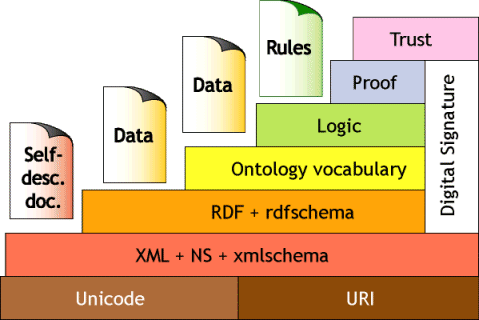
\includegraphics[scale=0.5]{layercake}
            \end{center}
            \begin{flushright}
                \texttt{[w3.org]}
            \end{flushright}
            This talk focuses on layers 3 and 4 
        \end{frame}


        \begin{frame}
            \frametitle{Syntax? Semantic?!?!?}

            While talking a lot about semantics and syntax\ldots\\
            \ldots what's this all about?
            \pause
            \vskip 0.3cm
            \textit{Syntax}\\
            Syntax means defining rules about the structure of data, i.e.\\
            the structure of words in phrases or how well formed XML looks like.
            \pause
            \vskip 0.3cm
            \textit{Semantic}\\
            Semantic in general defines the meanings of terms, sentences or XML-
            constructs.
            \pause
            \vskip 0.3cm
            For example, the word ``\textit{wine}'' has different meanings while beeing syntactically the same.
            It can represent a beverage or also a famous piece of software.
        \end{frame}

        \begin{frame}
            \frametitle{History}

            Important points in the history of the semantic web:
            \pause
            \vskip 0.7cm

            \begin{itemize}
                \item Some initial work during 1997-1998
                \pause
                \item In 1999
                    \pause
                    \begin{itemize}
                        \item February: First recommendation, RDF model and syntax
                        \pause
                        \item March: rdfschema proposal
                    \end{itemize}
                \pause
                \item February 2004: A suite of RDF and OWL recommendations, rdfschema recommendation
                \pause
                \item Most widely used since for RSS-feeds (but not known for that\ldots)
                \pause
                \item My first contact with it: 2003
            \end{itemize}
        \end{frame}




    \section{RDF}

        \begin{frame}
            \frametitle{Basic concepts}

            \textit{``Everything should be representable, so one needs a common model with great generality''}
            \vskip 0.3cm
            \textit{``Two basic elements:\\
            Assertions\\
            Quotations (statements about assertions)''}
            \vskip 0.3cm
            \begin{flushright}
                \texttt{[http://www.w3.org/DesignIssues/Semantic.html]}
            \end{flushright}
        \end{frame}


        \begin{frame}
            \frametitle{RDF model}

            This leads to a very simplistic model, to RDF:
            \vskip 0.7cm
            \pause

            \begin{itemize}
                \item Information is represented as a \textit{triple}, as a statement
                \pause
                \item Every triple consists of three elements:
                \pause
                \begin{itemize}
                    \item \textbf{Subject}
                    \pause
                    \item \textbf{Predicate}
                    \pause
                    \item \textbf{Object}
                    \pause
               \end{itemize}
               \item Subjects and predicates are given as URIs
               \pause
               \item Objects can either be other URIs or literal data
               \pause
               \item RDF data is represented by directed graphs 
           \end{itemize}
        \end{frame}

        \begin{frame}
            \frametitle{Example\ldots}

            Based on that knowledge, we can build a first example.
            \vskip 0.3cm
            Given the following natural language assumptions:
            \pause
            \vskip 0.5cm
            \textit{``Mary has a lamb.''\\
            \pause
            \textit{``Mary is 14.''}\\
            \pause
            ``Big bad wolf wants this lamb.''\\
            \pause
            ``Big bad wolf engages the seven dwarfs.''\\
            \pause
            ``The seven dwarfs must steal the lamb.''\\}
            \pause
            \ldots and of course\ldots\\
            \pause
            \textit{``the lamb is an animal!''}
            \pause
            \vskip 0.5cm
            Represented as a graph, this would look like\ldots
        \end{frame}

        \begin{frame}
            \frametitle{Example - graph}

            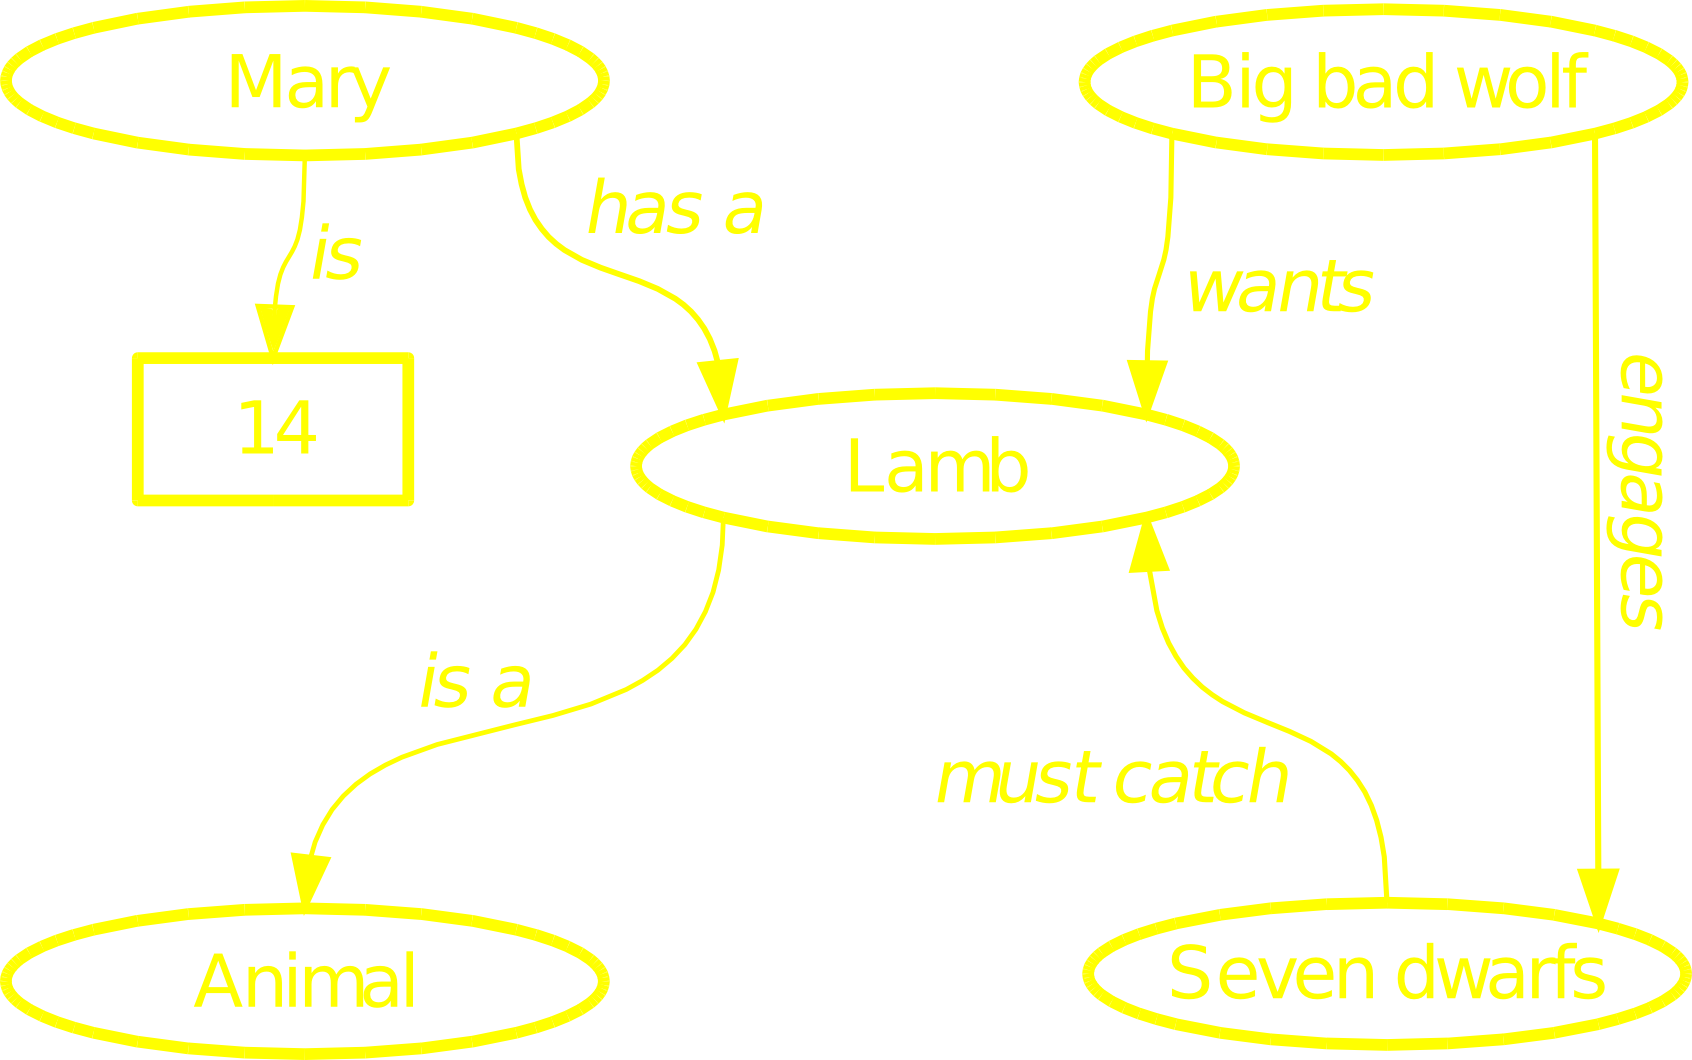
\includegraphics[scale=0.7]{graph}
        \end{frame}

        \begin{frame}
            \frametitle{Serialisation}

            Expressing triples as graphs is nice and comprehensible - for humans.
            But again - not very well parseable. Usually triples are handled in
            some serialized form. Multiple serialisation forms exist.
            \vskip 0.7cm
            \pause

            \begin{itemize}
                \item \textbf{Notation 3 (N3)} - first form, quite complex
                \pause
                \item \textbf{N-Triples} - subset of N3, possible recommendation
                \pause
                \item \textbf{Turtle} - extension of N3
                \pause
                \item \textbf{XML}
                \pause
           \end{itemize}
           \vskip 0.7cm
           Turtle and XML are the most used forms. Turtle is quite practical when writing
           triples by hand, XML of course in automated exchange.
       \end{frame}

       \begin{frame}
           \frametitle{Example - turtle serialisation 1}
           \footnotesize
           \texttt{\ding{229} <http://example.org/Mary>    <http://example.org/has>    <http://example.org/Lamb>  .\\
           \ding{229} <http://example.org/Mary>    <http://example.org/is>     ``14''  .\\
           \ding{229} <http://example.org/BigBadWolf>    <http://example.org/wants>   <http://example.org/Lamb>  .\\
           \ding{229} <http://example.org/BigBadWolf>    <http://example.org/engages>    <http://example.org/SevenDwarfs>  .\\
           \ding{229} <http://example.org/SevenDwarfs>    <http://example.org/muststeal>    <http://example.org/Lamb>  .\\
           \ding{229} <http://example.org/Lamb>    <http://example.org/isa>    <http://example.org/Animal>  .}
           \normalsize
           \vskip 0.7cm
           \textit{Note: lines are split up due to space. Each line starts with \ding{229}}
       \end{frame}

       \begin{frame}
           \frametitle{Example - turtle serialisation 2}
           Of course this isn't very handy, so here is a more cleaned up version:
           \footnotesize
           \vskip 0.7cm
           \texttt{\ding{229} @prefix ex: <http://example.org> . \\
           \ding{229} ex:Mary          ex:has          ex:Lamb ; \\
           \ding{229}                  ex:is           ``14''  . \\
           \ding{229} ex:BigBadWolf    ex:wants        ex:Lamb ; \\
           \ding{229}                  ex:engages      ex:SevenDwarfs  . \\           
           \ding{229} ex:SevenDwarfs   ex:muststeal    ex:Lamb . \\
           \ding{229} ex:Lamb          ex:isa          ex:Animal}
           \normalsize
           \vskip 0.7cm
           \textit{Note: Turtle provides also other shortcuts not shown here}
       \end{frame}

       \begin{frame}
           \frametitle{Example - XML serialisation}
           \vskip 0.8cm
           I will now show you this example serialised as XML.\\
           Unfortunately, I didn't have the time to fully remake it, so i took
           the one from the previous speech - but there are only a few things missing and
           it will be enough to demonstrate how it looks like\ldots
       \end{frame}
 
       \begin{frame}
           \frametitle{RDF - additional features}

           RDF provides additional features for added expressiveness
           \vskip 0.7cm
           \pause
           \begin{itemize}
               \item Typed literals: literals are identified by an URI, often used for XMLSchema-datatypes
               \pause
               \item Localisation of literals (language specific literals)
               \pause
               \item Empty nodes for complex relationships
               \pause
               \item Containers, lists, collections
               \pause
           \end{itemize}
           \vskip 0.7cm
           \textit{I won't cover these in this talk, please refer to additional literature.}
       \end{frame}


    \section{rdfschema}

       \begin{frame}
           \frametitle{rdfschema - simple ontologies}

           rdfschema can be used to describe simple \textbf{ontologies}.
           \vskip 0.3cm
           \pause
           An ontology is a \textit{network} of informations with logical relations.
           One can also think of it as ``knowledge in a jar'', an ontology
           usually covers one or more areas of knowledge.
           \vskip 0.3cm
           \pause
           As opposed to this, a \textbf{taxonomy} is \textit{hierarchically organised}.
           Example: In biology, the classification of a human as a mammal (with multiple
           levels inbetween of course), is a taxonomy.
       \end{frame}

       \begin{frame}
           \frametitle{rdfschema - simple ontologies}

           rdfschema provides basic mechanisms for structuring RDF data.
           \vskip 0.3cm
           \pause
           Often, the functions given by rdfschema will be sufficient for simple
           ontologies.
           \vskip 0.3cm
           \pause
           Dublin core is a well known rdfschema ontology.
       \end{frame}

       \begin{frame}
           \frametitle{Features of rdfschema}

           The most important constructs given by rdfschema are:
           \vskip 0.7cm
           \pause
           \begin{itemize}
               \item \texttt{rdfs:Class, rdfs:subClassOf}
               \pause
               \item \texttt{rdfs:Property, rdfs:subPropertyOf, rdfs:range, rdfs:domain}
               \pause
               \item \texttt{rdfs:type}
               \pause
               \item \texttt{rdfs:Container} (used for lists, sequences etc.)
           \end{itemize}
       \end{frame}

       \begin{frame}
           \frametitle{rdfschema - examples}

           Let's look at some examples (based on the tale of the lamb and the wolf\ldots):
           \vskip 0.7cm
           \pause
           \texttt{ex:Person    rdfs:subClassOf     <http://genome.org/human>}
           \vskip 0.3cm
           \pause
           \texttt{ex:Mary    rdfs:type     ex:Person}
           \vskip 0.3cm
           \pause
           \texttt{ex:is    rdfs:subPropertyOf    <http://older.net/ageproperty>}
           \vskip 0.3cm
           \pause
           \texttt{ex:is    rdfs:range      ex:Person}
           \vskip 0.7cm
           \pause
           Of course, these are only a few and very simple examples - I hope you get the idea!
       \end{frame}

    \section{OWL}

       \begin{frame}
           \frametitle{OWL - introduction}

           \textbf{OWL} is the \textbf{W}eb \textbf{O}ntology \textbf{L}anguage
           \vskip 0.3cm
           Yes, that would be \textbf{WOL} and not \textbf{OWL}! but\ldots
           \vskip 0.7cm
           \pause
           \begin{itemize}
               \item It's clear how to pronounce OWL\ldots
               \pause
               \item This acronym is great for making logos\ldots
               \pause
               \item OWLs are associated with wisdom\ldots
               \pause
               \item This makes up a great backstory\ldots
               \pause
           \end{itemize}
           \footnotesize  %TODO verbatim?
           \texttt{[http://lists.w3.org/Archives/Public/www-webont-wg/2001Dec/0169.html]} 
           \normalsize
           \pause
           \vskip 0.7cm
           A theory is also, that this comes from Winnie the Pooh, where the owl wasn't able to
           write her name correctly\ldots ;-)
       \end{frame}

       \begin{frame}
           \frametitle{OWL - variants}

           There are three different variants of OWL:\\
           \pause
           \textbf{OWL Full}\\
           \begin{itemize}
               \item Contains \textbf{OWL DL} and \textbf{OWL Lite}
               \item Very expressive
               \item Not decideable (that causes headaches to reasoners\ldots)
               \item Not fully supported by software
           \end{itemize}
           \pause
           \textbf{OWL DL}
           \begin{itemize}
               \item Contains \textbf{OWL Lite}
               \item Decideable
               \item Nearly fully software supported
           \end{itemize}
           \pause
           \textbf{OWL Lite}
           \begin{itemize}
               \item Decideable
               \item Fully software supported
               \item Less expressive
           \end{itemize}
       \end{frame}

       \begin{frame}
           \frametitle{OWL Lite - constructs}

           OWL Lite provides constructs for
           \vskip 0.7cm
           \begin{itemize}           
               \item (In-)Equality
               \item Property characteristics
               \item Property restrictions
               \item Cardinality restrictions
               \item Header informations
               \item Class intersections
               \item Versioning
               \item Annotation
               \item Datatypes
           \end{itemize}
           \vskip 0.7cm
           And of course, rdfschema can also be combined with OWL\ldots!
       \end{frame}

       \begin{frame}
           \frametitle{OWL Lite - constructs}

           Some example of OWL Lite constructs:
           \vskip 0.7cm
           \begin{itemize}
               \item \texttt{owl:equivalentClass, owl:equivalentProperty}
               \item \texttt{owl:ObjectProperty, owl:DatatypeProperty}
               \item \texttt{owl:minCardinality, owl:maxCardinality}
               \item \texttt{owl:intersectionOf}
               \item \texttt{owl:versionInfo}
               \item \texttt{owl:AnnotationProperty, owl:OntologyProperty}
           \end{itemize}
       \end{frame}

       \begin{frame}
           \frametitle{OWL DL/Full - constructs}

           Additionally, OWL DL and OWL Full introduce the following constructs:
           \vskip 0.7cm
           \begin{itemize}           
               \item oneOf
               \item dataRange
               \item disjointWith
               \item equivalentClass
               \item unionOf, complementOf
               \item maxCardinality, cardinality
               \item hasValue
           \end{itemize}
       \end{frame}

       \begin{frame}
           \frametitle{Full example}

           Let's have a look at a simple example which shows what has been discussed
           until now.
           \vskip 0.3cm
           This example has been taken from wikipedia.

       \end{frame}

       \begin{frame}
           \frametitle{What can be done now?}

           We've learned a lot about technologies so far - but how can this be used?
           \vskip 0.3cm
           \pause
           There are a lot of APIs out there for various languages, which help working
           with semantical information and ontologies. Examples include Jena (JAVA) and
           LibRDF (multiple languages).
           \vskip 0.3cm
           \pause
           Also, there is a multitude of triplestores. Triplestores are the databases for
           RDF-data, they store - as the name implies - triples.
           \vskip 0.3cm
           \pause
           \textit{Check out my links for more information\ldots!}
       \end{frame}

       \begin{frame}
           \frametitle{Querying}

           RDF data can also be queried. Recently, \textbf{SPARQL} has been defined as
           an official standard. 
           \vskip 0.3cm
           \pause
           Giving a broad introducion into SPARQL doesn't fit into the timeframe of this
           speech. I recommend you further reading on the web\ldots
       \end{frame}

       \begin{frame}
           \frametitle{Infering and Reasoning}

           Besides of that, also infering and reasoning are interesting and important
           applications of RDF.
           \vskip 0.3cm
           \pause
           You can understand those as making automatic assumptions about triples.
           As a (very simple) example, look at this:
           \vskip 0.3cm
           \pause
           \textit{When we know that all human beeings are born\ldots\\
           \ldots and we know that Pascal Mainini is a human beeing\ldots\\
           \ldots we can automatically infer that Pascal Mainini has been born!}
           \vskip 0.3cm
           \pause
           Reasoning and infering go into artificial intelligence. I won't go any
           further here too - but it's a very interesting field and you can - again
           find a lot of information and tools on the web!
       \end{frame}



    \section{Conclusion}

       \begin{frame}
           \frametitle{Conclusion}

           We are reaching the end of this speech\ldots\\
           I hope that:
           \vskip 0.7cm
           \pause
           \begin{itemize}
               \item This was interesting to you\ldots!
               \pause
               \item I was able to give you a good overview over this broad topic\ldots!
               \pause
               \item You will be able to start your own explorations - if you like to\ldots!
           \end{itemize}


       \end{frame}

       \begin{frame}
           \frametitle{Questions}

           Are there any\ldots
           \vskip 0.7cm
           \huge
           \ldots Questions?!?
           \normalsize

       \end{frame}

       \begin{frame}
           \frametitle{Thanks!}
           \vskip 0.7cm
           \huge
           Thanks a lot for your interest!
           \normalsize
           \vskip 0.7cm
           Check out 
           \vskip 0.5cm
           \texttt{http://impressionet.ch/semwebspeech2}
           \vskip 0.5cm
           by the end of next week to find all the information!
       \end{frame}

\end{document}

